% Created by tikzDevice version 0.12.3 on 2020-09-18 17:13:47
% !TEX encoding = UTF-8 Unicode
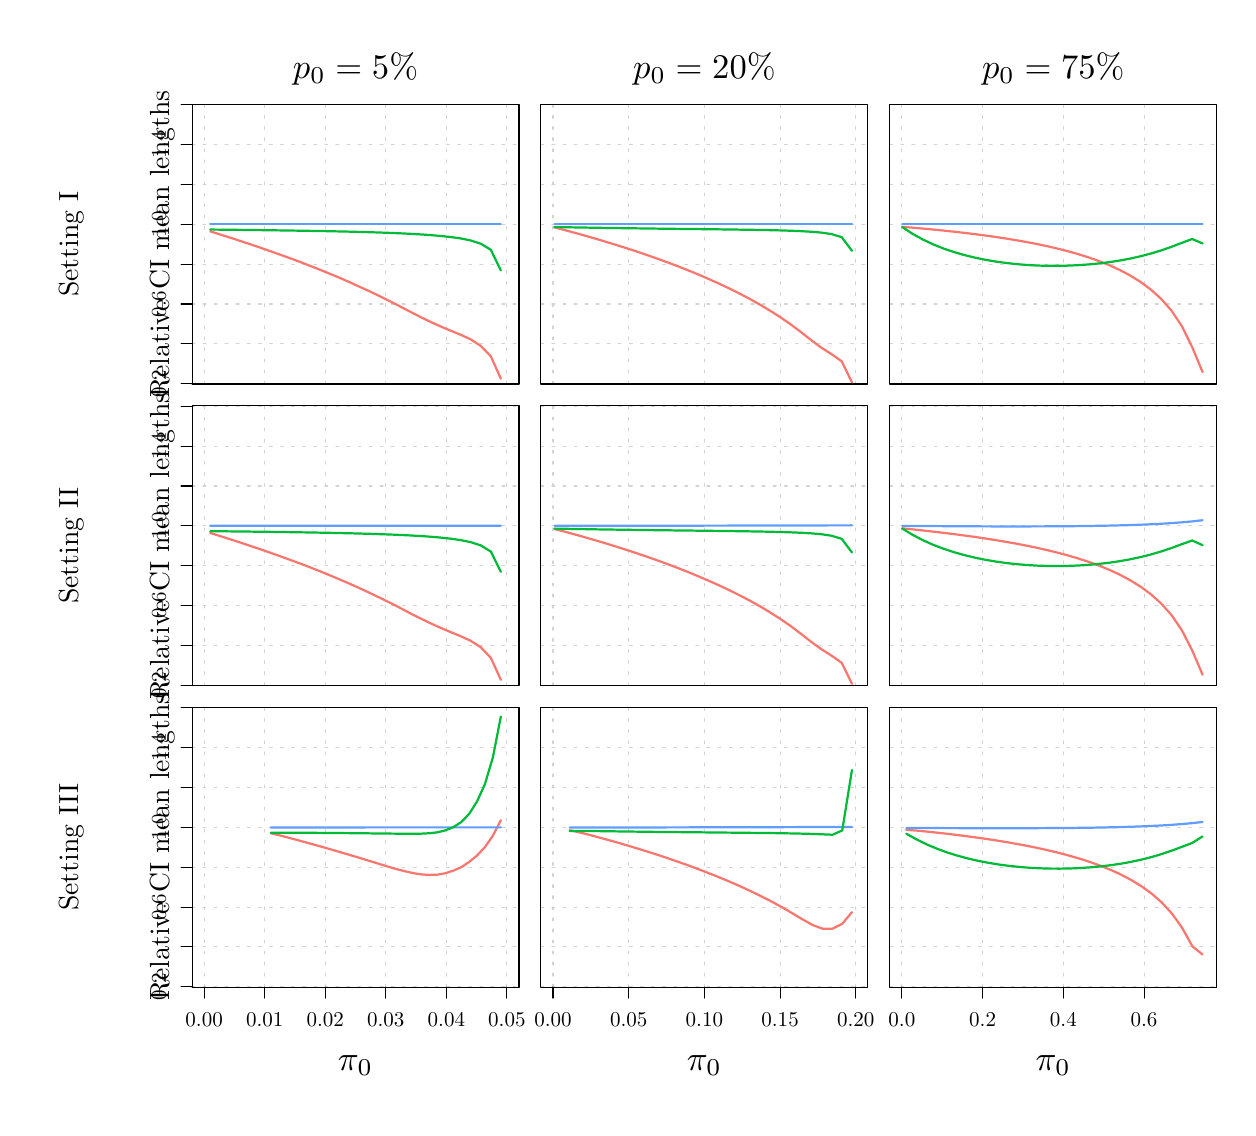
\begin{tikzpicture}[x=1pt,y=1pt]
\definecolor{fillColor}{RGB}{255,255,255}
\path[use as bounding box,fill=fillColor,fill opacity=0.00] (0,0) rectangle (433.62,390.26);
\begin{scope}
\path[clip] ( 55.44,257.53) rectangle (181.50,366.50);
\definecolor{drawColor}{RGB}{0,0,0}

\node[text=drawColor,anchor=base,inner sep=0pt, outer sep=0pt, scale=  0.66] at (118.47,231.40) {Simulation ID};

\node[text=drawColor,rotate= 90.00,anchor=base,inner sep=0pt, outer sep=0pt, scale=  0.66] at ( 34.06,312.01) {Ratio of RMSE};
\end{scope}
\begin{scope}
\path[clip] (  0.00,  0.00) rectangle (433.62,390.26);
\definecolor{drawColor}{RGB}{0,0,0}

\path[draw=drawColor,line width= 0.4pt,line join=round,line cap=round] ( 59.40,261.64) -- ( 59.40,362.39);

\path[draw=drawColor,line width= 0.4pt,line join=round,line cap=round] ( 59.40,261.64) -- ( 55.44,261.64);

\path[draw=drawColor,line width= 0.4pt,line join=round,line cap=round] ( 59.40,276.03) -- ( 55.44,276.03);

\path[draw=drawColor,line width= 0.4pt,line join=round,line cap=round] ( 59.40,290.42) -- ( 55.44,290.42);

\path[draw=drawColor,line width= 0.4pt,line join=round,line cap=round] ( 59.40,304.82) -- ( 55.44,304.82);

\path[draw=drawColor,line width= 0.4pt,line join=round,line cap=round] ( 59.40,319.21) -- ( 55.44,319.21);

\path[draw=drawColor,line width= 0.4pt,line join=round,line cap=round] ( 59.40,333.61) -- ( 55.44,333.61);

\path[draw=drawColor,line width= 0.4pt,line join=round,line cap=round] ( 59.40,348.00) -- ( 55.44,348.00);

\path[draw=drawColor,line width= 0.4pt,line join=round,line cap=round] ( 59.40,362.39) -- ( 55.44,362.39);

\node[text=drawColor,rotate= 90.00,anchor=base,inner sep=0pt, outer sep=0pt, scale=  0.76] at ( 49.90,261.64) {0.2};

\node[text=drawColor,rotate= 90.00,anchor=base,inner sep=0pt, outer sep=0pt, scale=  0.76] at ( 49.90,290.42) {0.6};

\node[text=drawColor,rotate= 90.00,anchor=base,inner sep=0pt, outer sep=0pt, scale=  0.76] at ( 49.90,319.21) {1.0};

\node[text=drawColor,rotate= 90.00,anchor=base,inner sep=0pt, outer sep=0pt, scale=  0.76] at ( 49.90,348.00) {1.4};
\end{scope}
\begin{scope}
\path[clip] ( 59.40,261.49) rectangle (177.54,362.54);
\definecolor{drawColor}{RGB}{211,211,211}

\path[draw=drawColor,line width= 0.4pt,dash pattern=on 1pt off 3pt ,line join=round,line cap=round] ( 63.78,261.49) -- ( 63.78,362.54);

\path[draw=drawColor,line width= 0.4pt,dash pattern=on 1pt off 3pt ,line join=round,line cap=round] ( 85.65,261.49) -- ( 85.65,362.54);

\path[draw=drawColor,line width= 0.4pt,dash pattern=on 1pt off 3pt ,line join=round,line cap=round] (107.53,261.49) -- (107.53,362.54);

\path[draw=drawColor,line width= 0.4pt,dash pattern=on 1pt off 3pt ,line join=round,line cap=round] (129.41,261.49) -- (129.41,362.54);

\path[draw=drawColor,line width= 0.4pt,dash pattern=on 1pt off 3pt ,line join=round,line cap=round] (151.29,261.49) -- (151.29,362.54);

\path[draw=drawColor,line width= 0.4pt,dash pattern=on 1pt off 3pt ,line join=round,line cap=round] (173.16,261.49) -- (173.16,362.54);

\path[draw=drawColor,line width= 0.4pt,dash pattern=on 1pt off 3pt ,line join=round,line cap=round] ( 59.40,261.64) -- (177.54,261.64);

\path[draw=drawColor,line width= 0.4pt,dash pattern=on 1pt off 3pt ,line join=round,line cap=round] ( 59.40,276.03) -- (177.54,276.03);

\path[draw=drawColor,line width= 0.4pt,dash pattern=on 1pt off 3pt ,line join=round,line cap=round] ( 59.40,290.42) -- (177.54,290.42);

\path[draw=drawColor,line width= 0.4pt,dash pattern=on 1pt off 3pt ,line join=round,line cap=round] ( 59.40,304.82) -- (177.54,304.82);

\path[draw=drawColor,line width= 0.4pt,dash pattern=on 1pt off 3pt ,line join=round,line cap=round] ( 59.40,319.21) -- (177.54,319.21);

\path[draw=drawColor,line width= 0.4pt,dash pattern=on 1pt off 3pt ,line join=round,line cap=round] ( 59.40,333.61) -- (177.54,333.61);

\path[draw=drawColor,line width= 0.4pt,dash pattern=on 1pt off 3pt ,line join=round,line cap=round] ( 59.40,348.00) -- (177.54,348.00);

\path[draw=drawColor,line width= 0.4pt,dash pattern=on 1pt off 3pt ,line join=round,line cap=round] ( 59.40,362.39) -- (177.54,362.39);
\end{scope}
\begin{scope}
\path[clip] (  0.00,  0.00) rectangle (433.62,390.26);
\definecolor{drawColor}{RGB}{0,0,0}

\path[draw=drawColor,line width= 0.4pt,line join=round,line cap=round] ( 59.40,261.49) --
	(177.54,261.49) --
	(177.54,362.54) --
	( 59.40,362.54) --
	( 59.40,261.49);
\end{scope}
\begin{scope}
\path[clip] ( 59.40,261.49) rectangle (177.54,362.54);
\definecolor{drawColor}{RGB}{248,118,109}

\path[draw=drawColor,line width= 0.8pt,line join=round,line cap=round] ( 65.96,316.65) --
	( 69.58,315.52) --
	( 73.21,314.37) --
	( 76.83,313.19) --
	( 80.45,311.99) --
	( 84.07,310.76) --
	( 87.69,309.50) --
	( 91.31,308.21) --
	( 94.93,306.90) --
	( 98.55,305.57) --
	(102.17,304.14) --
	(105.80,302.72) --
	(109.42,301.22) --
	(113.04,299.73) --
	(116.66,298.14) --
	(120.28,296.47) --
	(123.90,294.84) --
	(127.52,293.08) --
	(131.14,291.29) --
	(134.77,289.42) --
	(138.39,287.53) --
	(142.01,285.67) --
	(145.63,283.92) --
	(149.25,282.28) --
	(152.87,280.75) --
	(156.49,279.28) --
	(160.11,277.61) --
	(163.73,275.26) --
	(167.36,271.50) --
	(170.98,263.44);
\definecolor{drawColor}{RGB}{97,156,255}

\path[draw=drawColor,line width= 0.8pt,line join=round,line cap=round] ( 65.96,319.21) --
	( 69.58,319.21) --
	( 73.21,319.21) --
	( 76.83,319.21) --
	( 80.45,319.21) --
	( 84.07,319.21) --
	( 87.69,319.21) --
	( 91.31,319.21) --
	( 94.93,319.21) --
	( 98.55,319.21) --
	(102.17,319.21) --
	(105.80,319.21) --
	(109.42,319.21) --
	(113.04,319.21) --
	(116.66,319.21) --
	(120.28,319.21) --
	(123.90,319.21) --
	(127.52,319.21) --
	(131.14,319.21) --
	(134.77,319.21) --
	(138.39,319.21) --
	(142.01,319.21) --
	(145.63,319.21) --
	(149.25,319.21) --
	(152.87,319.21) --
	(156.49,319.21) --
	(160.11,319.21) --
	(163.73,319.21) --
	(167.36,319.21) --
	(170.98,319.21);
\definecolor{drawColor}{RGB}{0,186,56}

\path[draw=drawColor,line width= 0.8pt,line join=round,line cap=round] ( 65.96,317.30) --
	( 69.58,317.27) --
	( 73.21,317.23) --
	( 76.83,317.19) --
	( 80.45,317.14) --
	( 84.07,317.10) --
	( 87.69,317.05) --
	( 91.31,317.00) --
	( 94.93,316.95) --
	( 98.55,316.89) --
	(102.17,316.83) --
	(105.80,316.77) --
	(109.42,316.70) --
	(113.04,316.62) --
	(116.66,316.54) --
	(120.28,316.44) --
	(123.90,316.34) --
	(127.52,316.22) --
	(131.14,316.09) --
	(134.77,315.94) --
	(138.39,315.76) --
	(142.01,315.55) --
	(145.63,315.30) --
	(149.25,314.99) --
	(152.87,314.60) --
	(156.49,314.10) --
	(160.11,313.36) --
	(163.73,312.19) --
	(167.36,309.99) --
	(170.98,302.52);
\end{scope}
\begin{scope}
\path[clip] (  0.00,  0.00) rectangle (433.62,390.26);
\definecolor{drawColor}{RGB}{0,0,0}

\node[text=drawColor,rotate= 90.00,anchor=base,inner sep=0pt, outer sep=0pt, scale=  1.00] at ( 18.22,312.01) {Setting I};

\node[text=drawColor,rotate= 90.00,anchor=base,inner sep=0pt, outer sep=0pt, scale=  1.00] at ( 51.08,312.01) {Relative CI mean lengths};

\node[text=drawColor,anchor=base,inner sep=0pt, outer sep=0pt, scale=  1.25] at (118.47,372.04) {$p_0 = 5\%$};
\end{scope}
\begin{scope}
\path[clip] (181.50,257.53) rectangle (307.56,366.50);
\definecolor{drawColor}{RGB}{0,0,0}

\node[text=drawColor,anchor=base,inner sep=0pt, outer sep=0pt, scale=  0.66] at (244.53,231.40) {Simulation ID};

\node[text=drawColor,rotate= 90.00,anchor=base,inner sep=0pt, outer sep=0pt, scale=  0.66] at (160.12,312.01) {Ratio of RMSE};
\end{scope}
\begin{scope}
\path[clip] (185.46,261.49) rectangle (303.60,362.54);
\definecolor{drawColor}{RGB}{211,211,211}

\path[draw=drawColor,line width= 0.4pt,dash pattern=on 1pt off 3pt ,line join=round,line cap=round] (189.84,261.49) -- (189.84,362.54);

\path[draw=drawColor,line width= 0.4pt,dash pattern=on 1pt off 3pt ,line join=round,line cap=round] (217.18,261.49) -- (217.18,362.54);

\path[draw=drawColor,line width= 0.4pt,dash pattern=on 1pt off 3pt ,line join=round,line cap=round] (244.53,261.49) -- (244.53,362.54);

\path[draw=drawColor,line width= 0.4pt,dash pattern=on 1pt off 3pt ,line join=round,line cap=round] (271.88,261.49) -- (271.88,362.54);

\path[draw=drawColor,line width= 0.4pt,dash pattern=on 1pt off 3pt ,line join=round,line cap=round] (299.22,261.49) -- (299.22,362.54);

\path[draw=drawColor,line width= 0.4pt,dash pattern=on 1pt off 3pt ,line join=round,line cap=round] (185.46,261.64) -- (303.60,261.64);

\path[draw=drawColor,line width= 0.4pt,dash pattern=on 1pt off 3pt ,line join=round,line cap=round] (185.46,276.03) -- (303.60,276.03);

\path[draw=drawColor,line width= 0.4pt,dash pattern=on 1pt off 3pt ,line join=round,line cap=round] (185.46,290.42) -- (303.60,290.42);

\path[draw=drawColor,line width= 0.4pt,dash pattern=on 1pt off 3pt ,line join=round,line cap=round] (185.46,304.82) -- (303.60,304.82);

\path[draw=drawColor,line width= 0.4pt,dash pattern=on 1pt off 3pt ,line join=round,line cap=round] (185.46,319.21) -- (303.60,319.21);

\path[draw=drawColor,line width= 0.4pt,dash pattern=on 1pt off 3pt ,line join=round,line cap=round] (185.46,333.61) -- (303.60,333.61);

\path[draw=drawColor,line width= 0.4pt,dash pattern=on 1pt off 3pt ,line join=round,line cap=round] (185.46,348.00) -- (303.60,348.00);

\path[draw=drawColor,line width= 0.4pt,dash pattern=on 1pt off 3pt ,line join=round,line cap=round] (185.46,362.39) -- (303.60,362.39);
\end{scope}
\begin{scope}
\path[clip] (  0.00,  0.00) rectangle (433.62,390.26);
\definecolor{drawColor}{RGB}{0,0,0}

\path[draw=drawColor,line width= 0.4pt,line join=round,line cap=round] (185.46,261.49) --
	(303.60,261.49) --
	(303.60,362.54) --
	(185.46,362.54) --
	(185.46,261.49);
\end{scope}
\begin{scope}
\path[clip] (185.46,261.49) rectangle (303.60,362.54);
\definecolor{drawColor}{RGB}{248,118,109}

\path[draw=drawColor,line width= 0.8pt,line join=round,line cap=round] (190.38,318.09) --
	(194.09,317.11) --
	(197.79,316.10) --
	(201.50,315.06) --
	(205.21,314.00) --
	(208.91,312.89) --
	(212.62,311.76) --
	(216.32,310.59) --
	(220.03,309.38) --
	(223.74,308.12) --
	(227.44,306.82) --
	(231.15,305.47) --
	(234.85,304.07) --
	(238.56,302.61) --
	(242.27,301.09) --
	(245.97,299.49) --
	(249.68,297.84) --
	(253.38,296.09) --
	(257.09,294.24) --
	(260.80,292.31) --
	(264.50,290.24) --
	(268.21,288.03) --
	(271.91,285.66) --
	(275.62,283.12) --
	(279.33,280.32) --
	(283.03,277.41) --
	(286.74,274.65) --
	(290.45,272.29) --
	(294.15,269.69) --
	(297.86,262.07);
\definecolor{drawColor}{RGB}{97,156,255}

\path[draw=drawColor,line width= 0.8pt,line join=round,line cap=round] (190.38,319.21) --
	(194.09,319.21) --
	(197.79,319.21) --
	(201.50,319.21) --
	(205.21,319.21) --
	(208.91,319.21) --
	(212.62,319.21) --
	(216.32,319.21) --
	(220.03,319.21) --
	(223.74,319.21) --
	(227.44,319.21) --
	(231.15,319.21) --
	(234.85,319.21) --
	(238.56,319.21) --
	(242.27,319.21) --
	(245.97,319.21) --
	(249.68,319.21) --
	(253.38,319.21) --
	(257.09,319.21) --
	(260.80,319.21) --
	(264.50,319.21) --
	(268.21,319.21) --
	(271.91,319.21) --
	(275.62,319.21) --
	(279.33,319.21) --
	(283.03,319.21) --
	(286.74,319.21) --
	(290.45,319.21) --
	(294.15,319.21) --
	(297.86,319.21);
\definecolor{drawColor}{RGB}{0,186,56}

\path[draw=drawColor,line width= 0.8pt,line join=round,line cap=round] (190.38,318.22) --
	(194.09,318.15) --
	(197.79,318.08) --
	(201.50,318.02) --
	(205.21,317.95) --
	(208.91,317.90) --
	(212.62,317.84) --
	(216.32,317.79) --
	(220.03,317.74) --
	(223.74,317.69) --
	(227.44,317.64) --
	(231.15,317.59) --
	(234.85,317.55) --
	(238.56,317.51) --
	(242.27,317.47) --
	(245.97,317.42) --
	(249.68,317.38) --
	(253.38,317.33) --
	(257.09,317.28) --
	(260.80,317.23) --
	(264.50,317.16) --
	(268.21,317.09) --
	(271.91,317.00) --
	(275.62,316.88) --
	(279.33,316.73) --
	(283.03,316.52) --
	(286.74,316.21) --
	(290.45,315.68) --
	(294.15,314.56) --
	(297.86,309.61);
\end{scope}
\begin{scope}
\path[clip] (  0.00,  0.00) rectangle (433.62,390.26);
\definecolor{drawColor}{RGB}{0,0,0}

\node[text=drawColor,anchor=base,inner sep=0pt, outer sep=0pt, scale=  1.25] at (244.53,372.04) {$p_0 = 20\%$};
\end{scope}
\begin{scope}
\path[clip] (307.56,257.53) rectangle (433.62,366.50);
\definecolor{drawColor}{RGB}{0,0,0}

\node[text=drawColor,anchor=base,inner sep=0pt, outer sep=0pt, scale=  0.66] at (370.59,231.40) {Simulation ID};

\node[text=drawColor,rotate= 90.00,anchor=base,inner sep=0pt, outer sep=0pt, scale=  0.66] at (286.18,312.01) {Ratio of RMSE};
\end{scope}
\begin{scope}
\path[clip] (311.52,261.49) rectangle (429.66,362.54);
\definecolor{drawColor}{RGB}{211,211,211}

\path[draw=drawColor,line width= 0.4pt,dash pattern=on 1pt off 3pt ,line join=round,line cap=round] (315.90,261.49) -- (315.90,362.54);

\path[draw=drawColor,line width= 0.4pt,dash pattern=on 1pt off 3pt ,line join=round,line cap=round] (345.07,261.49) -- (345.07,362.54);

\path[draw=drawColor,line width= 0.4pt,dash pattern=on 1pt off 3pt ,line join=round,line cap=round] (374.24,261.49) -- (374.24,362.54);

\path[draw=drawColor,line width= 0.4pt,dash pattern=on 1pt off 3pt ,line join=round,line cap=round] (403.41,261.49) -- (403.41,362.54);

\path[draw=drawColor,line width= 0.4pt,dash pattern=on 1pt off 3pt ,line join=round,line cap=round] (311.52,261.64) -- (429.66,261.64);

\path[draw=drawColor,line width= 0.4pt,dash pattern=on 1pt off 3pt ,line join=round,line cap=round] (311.52,276.03) -- (429.66,276.03);

\path[draw=drawColor,line width= 0.4pt,dash pattern=on 1pt off 3pt ,line join=round,line cap=round] (311.52,290.42) -- (429.66,290.42);

\path[draw=drawColor,line width= 0.4pt,dash pattern=on 1pt off 3pt ,line join=round,line cap=round] (311.52,304.82) -- (429.66,304.82);

\path[draw=drawColor,line width= 0.4pt,dash pattern=on 1pt off 3pt ,line join=round,line cap=round] (311.52,319.21) -- (429.66,319.21);

\path[draw=drawColor,line width= 0.4pt,dash pattern=on 1pt off 3pt ,line join=round,line cap=round] (311.52,333.61) -- (429.66,333.61);

\path[draw=drawColor,line width= 0.4pt,dash pattern=on 1pt off 3pt ,line join=round,line cap=round] (311.52,348.00) -- (429.66,348.00);

\path[draw=drawColor,line width= 0.4pt,dash pattern=on 1pt off 3pt ,line join=round,line cap=round] (311.52,362.39) -- (429.66,362.39);
\end{scope}
\begin{scope}
\path[clip] (  0.00,  0.00) rectangle (433.62,390.26);
\definecolor{drawColor}{RGB}{0,0,0}

\path[draw=drawColor,line width= 0.4pt,line join=round,line cap=round] (311.52,261.49) --
	(429.66,261.49) --
	(429.66,362.54) --
	(311.52,362.54) --
	(311.52,261.49);
\end{scope}
\begin{scope}
\path[clip] (311.52,261.49) rectangle (429.66,362.54);
\definecolor{drawColor}{RGB}{248,118,109}

\path[draw=drawColor,line width= 0.8pt,line join=round,line cap=round] (316.04,318.30) --
	(319.78,317.99) --
	(323.53,317.66) --
	(327.27,317.31) --
	(331.01,316.93) --
	(334.75,316.53) --
	(338.49,316.11) --
	(342.23,315.65) --
	(345.98,315.16) --
	(349.72,314.64) --
	(353.46,314.07) --
	(357.20,313.46) --
	(360.94,312.80) --
	(364.69,312.08) --
	(368.43,311.29) --
	(372.17,310.42) --
	(375.91,309.47) --
	(379.65,308.42) --
	(383.39,307.23) --
	(387.14,305.91) --
	(390.88,304.42) --
	(394.62,302.70) --
	(398.36,300.72) --
	(402.10,298.40) --
	(405.85,295.63) --
	(409.59,292.24) --
	(413.33,287.99) --
	(417.07,282.38) --
	(420.81,274.78) --
	(424.56,265.78);
\definecolor{drawColor}{RGB}{97,156,255}

\path[draw=drawColor,line width= 0.8pt,line join=round,line cap=round] (316.04,319.21) --
	(319.78,319.21) --
	(323.53,319.21) --
	(327.27,319.21) --
	(331.01,319.21) --
	(334.75,319.21) --
	(338.49,319.21) --
	(342.23,319.21) --
	(345.98,319.21) --
	(349.72,319.21) --
	(353.46,319.21) --
	(357.20,319.21) --
	(360.94,319.21) --
	(364.69,319.21) --
	(368.43,319.21) --
	(372.17,319.21) --
	(375.91,319.21) --
	(379.65,319.21) --
	(383.39,319.21) --
	(387.14,319.21) --
	(390.88,319.21) --
	(394.62,319.21) --
	(398.36,319.21) --
	(402.10,319.21) --
	(405.85,319.21) --
	(409.59,319.21) --
	(413.33,319.21) --
	(417.07,319.21) --
	(420.81,319.21) --
	(424.56,319.21);
\definecolor{drawColor}{RGB}{0,186,56}

\path[draw=drawColor,line width= 0.8pt,line join=round,line cap=round] (316.04,318.21) --
	(319.78,315.75) --
	(323.53,313.68) --
	(327.27,311.92) --
	(331.01,310.43) --
	(334.75,309.17) --
	(338.49,308.08) --
	(342.23,307.17) --
	(345.98,306.40) --
	(349.72,305.76) --
	(353.46,305.24) --
	(357.20,304.83) --
	(360.94,304.52) --
	(364.69,304.31) --
	(368.43,304.20) --
	(372.17,304.19) --
	(375.91,304.27) --
	(379.65,304.44) --
	(383.39,304.70) --
	(387.14,305.07) --
	(390.88,305.52) --
	(394.62,306.11) --
	(398.36,306.81) --
	(402.10,307.65) --
	(405.85,308.64) --
	(409.59,309.77) --
	(413.33,311.07) --
	(417.07,312.51) --
	(420.81,313.89) --
	(424.56,312.27);
\end{scope}
\begin{scope}
\path[clip] (  0.00,  0.00) rectangle (433.62,390.26);
\definecolor{drawColor}{RGB}{0,0,0}

\node[text=drawColor,anchor=base,inner sep=0pt, outer sep=0pt, scale=  1.25] at (370.59,372.04) {$p_0 = 75\%$};
\end{scope}
\begin{scope}
\path[clip] ( 55.44,148.57) rectangle (181.50,257.53);
\definecolor{drawColor}{RGB}{0,0,0}

\node[text=drawColor,anchor=base,inner sep=0pt, outer sep=0pt, scale=  0.66] at (118.47,122.43) {Simulation ID};

\node[text=drawColor,rotate= 90.00,anchor=base,inner sep=0pt, outer sep=0pt, scale=  0.66] at ( 34.06,203.05) {Ratio of RMSE};
\end{scope}
\begin{scope}
\path[clip] (  0.00,  0.00) rectangle (433.62,390.26);
\definecolor{drawColor}{RGB}{0,0,0}

\path[draw=drawColor,line width= 0.4pt,line join=round,line cap=round] ( 59.40,152.67) -- ( 59.40,253.43);

\path[draw=drawColor,line width= 0.4pt,line join=round,line cap=round] ( 59.40,152.67) -- ( 55.44,152.67);

\path[draw=drawColor,line width= 0.4pt,line join=round,line cap=round] ( 59.40,167.06) -- ( 55.44,167.06);

\path[draw=drawColor,line width= 0.4pt,line join=round,line cap=round] ( 59.40,181.46) -- ( 55.44,181.46);

\path[draw=drawColor,line width= 0.4pt,line join=round,line cap=round] ( 59.40,195.85) -- ( 55.44,195.85);

\path[draw=drawColor,line width= 0.4pt,line join=round,line cap=round] ( 59.40,210.25) -- ( 55.44,210.25);

\path[draw=drawColor,line width= 0.4pt,line join=round,line cap=round] ( 59.40,224.64) -- ( 55.44,224.64);

\path[draw=drawColor,line width= 0.4pt,line join=round,line cap=round] ( 59.40,239.03) -- ( 55.44,239.03);

\path[draw=drawColor,line width= 0.4pt,line join=round,line cap=round] ( 59.40,253.43) -- ( 55.44,253.43);

\node[text=drawColor,rotate= 90.00,anchor=base,inner sep=0pt, outer sep=0pt, scale=  0.76] at ( 49.90,152.67) {0.2};

\node[text=drawColor,rotate= 90.00,anchor=base,inner sep=0pt, outer sep=0pt, scale=  0.76] at ( 49.90,181.46) {0.6};

\node[text=drawColor,rotate= 90.00,anchor=base,inner sep=0pt, outer sep=0pt, scale=  0.76] at ( 49.90,210.25) {1.0};

\node[text=drawColor,rotate= 90.00,anchor=base,inner sep=0pt, outer sep=0pt, scale=  0.76] at ( 49.90,239.03) {1.4};
\end{scope}
\begin{scope}
\path[clip] ( 59.40,152.53) rectangle (177.54,253.57);
\definecolor{drawColor}{RGB}{211,211,211}

\path[draw=drawColor,line width= 0.4pt,dash pattern=on 1pt off 3pt ,line join=round,line cap=round] ( 63.78,152.53) -- ( 63.78,253.57);

\path[draw=drawColor,line width= 0.4pt,dash pattern=on 1pt off 3pt ,line join=round,line cap=round] ( 85.65,152.53) -- ( 85.65,253.57);

\path[draw=drawColor,line width= 0.4pt,dash pattern=on 1pt off 3pt ,line join=round,line cap=round] (107.53,152.53) -- (107.53,253.57);

\path[draw=drawColor,line width= 0.4pt,dash pattern=on 1pt off 3pt ,line join=round,line cap=round] (129.41,152.53) -- (129.41,253.57);

\path[draw=drawColor,line width= 0.4pt,dash pattern=on 1pt off 3pt ,line join=round,line cap=round] (151.29,152.53) -- (151.29,253.57);

\path[draw=drawColor,line width= 0.4pt,dash pattern=on 1pt off 3pt ,line join=round,line cap=round] (173.16,152.53) -- (173.16,253.57);

\path[draw=drawColor,line width= 0.4pt,dash pattern=on 1pt off 3pt ,line join=round,line cap=round] ( 59.40,152.67) -- (177.54,152.67);

\path[draw=drawColor,line width= 0.4pt,dash pattern=on 1pt off 3pt ,line join=round,line cap=round] ( 59.40,167.06) -- (177.54,167.06);

\path[draw=drawColor,line width= 0.4pt,dash pattern=on 1pt off 3pt ,line join=round,line cap=round] ( 59.40,181.46) -- (177.54,181.46);

\path[draw=drawColor,line width= 0.4pt,dash pattern=on 1pt off 3pt ,line join=round,line cap=round] ( 59.40,195.85) -- (177.54,195.85);

\path[draw=drawColor,line width= 0.4pt,dash pattern=on 1pt off 3pt ,line join=round,line cap=round] ( 59.40,210.25) -- (177.54,210.25);

\path[draw=drawColor,line width= 0.4pt,dash pattern=on 1pt off 3pt ,line join=round,line cap=round] ( 59.40,224.64) -- (177.54,224.64);

\path[draw=drawColor,line width= 0.4pt,dash pattern=on 1pt off 3pt ,line join=round,line cap=round] ( 59.40,239.03) -- (177.54,239.03);

\path[draw=drawColor,line width= 0.4pt,dash pattern=on 1pt off 3pt ,line join=round,line cap=round] ( 59.40,253.43) -- (177.54,253.43);
\end{scope}
\begin{scope}
\path[clip] (  0.00,  0.00) rectangle (433.62,390.26);
\definecolor{drawColor}{RGB}{0,0,0}

\path[draw=drawColor,line width= 0.4pt,line join=round,line cap=round] ( 59.40,152.53) --
	(177.54,152.53) --
	(177.54,253.57) --
	( 59.40,253.57) --
	( 59.40,152.53);
\end{scope}
\begin{scope}
\path[clip] ( 59.40,152.53) rectangle (177.54,253.57);
\definecolor{drawColor}{RGB}{248,118,109}

\path[draw=drawColor,line width= 0.8pt,line join=round,line cap=round] ( 65.96,207.67) --
	( 69.58,206.53) --
	( 73.21,205.38) --
	( 76.83,204.21) --
	( 80.45,203.01) --
	( 84.07,201.78) --
	( 87.69,200.52) --
	( 91.31,199.24) --
	( 94.93,197.91) --
	( 98.55,196.59) --
	(102.17,195.20) --
	(105.80,193.75) --
	(109.42,192.27) --
	(113.04,190.74) --
	(116.66,189.19) --
	(120.28,187.55) --
	(123.90,185.87) --
	(127.52,184.12) --
	(131.14,182.35) --
	(134.77,180.49) --
	(138.39,178.56) --
	(142.01,176.76) --
	(145.63,175.01) --
	(149.25,173.37) --
	(152.87,171.85) --
	(156.49,170.35) --
	(160.11,168.69) --
	(163.73,166.37) --
	(167.36,162.55) --
	(170.98,154.61);
\definecolor{drawColor}{RGB}{97,156,255}

\path[draw=drawColor,line width= 0.8pt,line join=round,line cap=round] ( 65.96,210.25) --
	( 69.58,210.25) --
	( 73.21,210.25) --
	( 76.83,210.25) --
	( 80.45,210.25) --
	( 84.07,210.25) --
	( 87.69,210.25) --
	( 91.31,210.25) --
	( 94.93,210.26) --
	( 98.55,210.26) --
	(102.17,210.26) --
	(105.80,210.26) --
	(109.42,210.26) --
	(113.04,210.26) --
	(116.66,210.26) --
	(120.28,210.26) --
	(123.90,210.27) --
	(127.52,210.27) --
	(131.14,210.27) --
	(134.77,210.27) --
	(138.39,210.27) --
	(142.01,210.27) --
	(145.63,210.27) --
	(149.25,210.27) --
	(152.87,210.28) --
	(156.49,210.28) --
	(160.11,210.28) --
	(163.73,210.28) --
	(167.36,210.28) --
	(170.98,210.28);
\definecolor{drawColor}{RGB}{0,186,56}

\path[draw=drawColor,line width= 0.8pt,line join=round,line cap=round] ( 65.96,208.32) --
	( 69.58,208.28) --
	( 73.21,208.24) --
	( 76.83,208.20) --
	( 80.45,208.16) --
	( 84.07,208.11) --
	( 87.69,208.07) --
	( 91.31,208.02) --
	( 94.93,207.96) --
	( 98.55,207.90) --
	(102.17,207.85) --
	(105.80,207.78) --
	(109.42,207.71) --
	(113.04,207.63) --
	(116.66,207.55) --
	(120.28,207.45) --
	(123.90,207.35) --
	(127.52,207.23) --
	(131.14,207.10) --
	(134.77,206.95) --
	(138.39,206.77) --
	(142.01,206.56) --
	(145.63,206.31) --
	(149.25,206.00) --
	(152.87,205.60) --
	(156.49,205.08) --
	(160.11,204.34) --
	(163.73,203.17) --
	(167.36,200.95) --
	(170.98,193.63);
\end{scope}
\begin{scope}
\path[clip] (  0.00,  0.00) rectangle (433.62,390.26);
\definecolor{drawColor}{RGB}{0,0,0}

\node[text=drawColor,rotate= 90.00,anchor=base,inner sep=0pt, outer sep=0pt, scale=  1.00] at ( 18.22,203.05) {Setting II};

\node[text=drawColor,rotate= 90.00,anchor=base,inner sep=0pt, outer sep=0pt, scale=  1.00] at ( 51.08,203.05) {Relative CI mean lengths};
\end{scope}
\begin{scope}
\path[clip] (181.50,148.57) rectangle (307.56,257.53);
\definecolor{drawColor}{RGB}{0,0,0}

\node[text=drawColor,anchor=base,inner sep=0pt, outer sep=0pt, scale=  0.66] at (244.53,122.43) {Simulation ID};

\node[text=drawColor,rotate= 90.00,anchor=base,inner sep=0pt, outer sep=0pt, scale=  0.66] at (160.12,203.05) {Ratio of RMSE};
\end{scope}
\begin{scope}
\path[clip] (185.46,152.53) rectangle (303.60,253.57);
\definecolor{drawColor}{RGB}{211,211,211}

\path[draw=drawColor,line width= 0.4pt,dash pattern=on 1pt off 3pt ,line join=round,line cap=round] (189.84,152.53) -- (189.84,253.57);

\path[draw=drawColor,line width= 0.4pt,dash pattern=on 1pt off 3pt ,line join=round,line cap=round] (217.18,152.53) -- (217.18,253.57);

\path[draw=drawColor,line width= 0.4pt,dash pattern=on 1pt off 3pt ,line join=round,line cap=round] (244.53,152.53) -- (244.53,253.57);

\path[draw=drawColor,line width= 0.4pt,dash pattern=on 1pt off 3pt ,line join=round,line cap=round] (271.88,152.53) -- (271.88,253.57);

\path[draw=drawColor,line width= 0.4pt,dash pattern=on 1pt off 3pt ,line join=round,line cap=round] (299.22,152.53) -- (299.22,253.57);

\path[draw=drawColor,line width= 0.4pt,dash pattern=on 1pt off 3pt ,line join=round,line cap=round] (185.46,152.67) -- (303.60,152.67);

\path[draw=drawColor,line width= 0.4pt,dash pattern=on 1pt off 3pt ,line join=round,line cap=round] (185.46,167.06) -- (303.60,167.06);

\path[draw=drawColor,line width= 0.4pt,dash pattern=on 1pt off 3pt ,line join=round,line cap=round] (185.46,181.46) -- (303.60,181.46);

\path[draw=drawColor,line width= 0.4pt,dash pattern=on 1pt off 3pt ,line join=round,line cap=round] (185.46,195.85) -- (303.60,195.85);

\path[draw=drawColor,line width= 0.4pt,dash pattern=on 1pt off 3pt ,line join=round,line cap=round] (185.46,210.25) -- (303.60,210.25);

\path[draw=drawColor,line width= 0.4pt,dash pattern=on 1pt off 3pt ,line join=round,line cap=round] (185.46,224.64) -- (303.60,224.64);

\path[draw=drawColor,line width= 0.4pt,dash pattern=on 1pt off 3pt ,line join=round,line cap=round] (185.46,239.03) -- (303.60,239.03);

\path[draw=drawColor,line width= 0.4pt,dash pattern=on 1pt off 3pt ,line join=round,line cap=round] (185.46,253.43) -- (303.60,253.43);
\end{scope}
\begin{scope}
\path[clip] (  0.00,  0.00) rectangle (433.62,390.26);
\definecolor{drawColor}{RGB}{0,0,0}

\path[draw=drawColor,line width= 0.4pt,line join=round,line cap=round] (185.46,152.53) --
	(303.60,152.53) --
	(303.60,253.57) --
	(185.46,253.57) --
	(185.46,152.53);
\end{scope}
\begin{scope}
\path[clip] (185.46,152.53) rectangle (303.60,253.57);
\definecolor{drawColor}{RGB}{248,118,109}

\path[draw=drawColor,line width= 0.8pt,line join=round,line cap=round] (190.38,209.11) --
	(194.09,208.13) --
	(197.79,207.12) --
	(201.50,206.07) --
	(205.21,205.00) --
	(208.91,203.90) --
	(212.62,202.75) --
	(216.32,201.57) --
	(220.03,200.36) --
	(223.74,199.10) --
	(227.44,197.79) --
	(231.15,196.44) --
	(234.85,195.04) --
	(238.56,193.58) --
	(242.27,192.05) --
	(245.97,190.46) --
	(249.68,188.81) --
	(253.38,187.07) --
	(257.09,185.23) --
	(260.80,183.29) --
	(264.50,181.23) --
	(268.21,179.01) --
	(271.91,176.65) --
	(275.62,174.10) --
	(279.33,171.31) --
	(283.03,168.40) --
	(286.74,165.70) --
	(290.45,163.36) --
	(294.15,160.74) --
	(297.86,153.15);
\definecolor{drawColor}{RGB}{97,156,255}

\path[draw=drawColor,line width= 0.8pt,line join=round,line cap=round] (190.38,210.25) --
	(194.09,210.25) --
	(197.79,210.25) --
	(201.50,210.26) --
	(205.21,210.26) --
	(208.91,210.27) --
	(212.62,210.27) --
	(216.32,210.28) --
	(220.03,210.28) --
	(223.74,210.29) --
	(227.44,210.29) --
	(231.15,210.30) --
	(234.85,210.30) --
	(238.56,210.31) --
	(242.27,210.31) --
	(245.97,210.32) --
	(249.68,210.32) --
	(253.38,210.33) --
	(257.09,210.34) --
	(260.80,210.34) --
	(264.50,210.35) --
	(268.21,210.36) --
	(271.91,210.36) --
	(275.62,210.37) --
	(279.33,210.38) --
	(283.03,210.39) --
	(286.74,210.40) --
	(290.45,210.41) --
	(294.15,210.41) --
	(297.86,210.42);
\definecolor{drawColor}{RGB}{0,186,56}

\path[draw=drawColor,line width= 0.8pt,line join=round,line cap=round] (190.38,209.25) --
	(194.09,209.18) --
	(197.79,209.11) --
	(201.50,209.05) --
	(205.21,208.98) --
	(208.91,208.92) --
	(212.62,208.87) --
	(216.32,208.82) --
	(220.03,208.77) --
	(223.74,208.72) --
	(227.44,208.67) --
	(231.15,208.63) --
	(234.85,208.58) --
	(238.56,208.54) --
	(242.27,208.50) --
	(245.97,208.45) --
	(249.68,208.41) --
	(253.38,208.36) --
	(257.09,208.31) --
	(260.80,208.25) --
	(264.50,208.19) --
	(268.21,208.11) --
	(271.91,208.02) --
	(275.62,207.90) --
	(279.33,207.75) --
	(283.03,207.54) --
	(286.74,207.22) --
	(290.45,206.68) --
	(294.15,205.55) --
	(297.86,200.60);
\end{scope}
\begin{scope}
\path[clip] (307.56,148.57) rectangle (433.62,257.53);
\definecolor{drawColor}{RGB}{0,0,0}

\node[text=drawColor,anchor=base,inner sep=0pt, outer sep=0pt, scale=  0.66] at (370.59,122.43) {Simulation ID};

\node[text=drawColor,rotate= 90.00,anchor=base,inner sep=0pt, outer sep=0pt, scale=  0.66] at (286.18,203.05) {Ratio of RMSE};
\end{scope}
\begin{scope}
\path[clip] (311.52,152.53) rectangle (429.66,253.57);
\definecolor{drawColor}{RGB}{211,211,211}

\path[draw=drawColor,line width= 0.4pt,dash pattern=on 1pt off 3pt ,line join=round,line cap=round] (315.90,152.53) -- (315.90,253.57);

\path[draw=drawColor,line width= 0.4pt,dash pattern=on 1pt off 3pt ,line join=round,line cap=round] (345.07,152.53) -- (345.07,253.57);

\path[draw=drawColor,line width= 0.4pt,dash pattern=on 1pt off 3pt ,line join=round,line cap=round] (374.24,152.53) -- (374.24,253.57);

\path[draw=drawColor,line width= 0.4pt,dash pattern=on 1pt off 3pt ,line join=round,line cap=round] (403.41,152.53) -- (403.41,253.57);

\path[draw=drawColor,line width= 0.4pt,dash pattern=on 1pt off 3pt ,line join=round,line cap=round] (311.52,152.67) -- (429.66,152.67);

\path[draw=drawColor,line width= 0.4pt,dash pattern=on 1pt off 3pt ,line join=round,line cap=round] (311.52,167.06) -- (429.66,167.06);

\path[draw=drawColor,line width= 0.4pt,dash pattern=on 1pt off 3pt ,line join=round,line cap=round] (311.52,181.46) -- (429.66,181.46);

\path[draw=drawColor,line width= 0.4pt,dash pattern=on 1pt off 3pt ,line join=round,line cap=round] (311.52,195.85) -- (429.66,195.85);

\path[draw=drawColor,line width= 0.4pt,dash pattern=on 1pt off 3pt ,line join=round,line cap=round] (311.52,210.25) -- (429.66,210.25);

\path[draw=drawColor,line width= 0.4pt,dash pattern=on 1pt off 3pt ,line join=round,line cap=round] (311.52,224.64) -- (429.66,224.64);

\path[draw=drawColor,line width= 0.4pt,dash pattern=on 1pt off 3pt ,line join=round,line cap=round] (311.52,239.03) -- (429.66,239.03);

\path[draw=drawColor,line width= 0.4pt,dash pattern=on 1pt off 3pt ,line join=round,line cap=round] (311.52,253.43) -- (429.66,253.43);
\end{scope}
\begin{scope}
\path[clip] (  0.00,  0.00) rectangle (433.62,390.26);
\definecolor{drawColor}{RGB}{0,0,0}

\path[draw=drawColor,line width= 0.4pt,line join=round,line cap=round] (311.52,152.53) --
	(429.66,152.53) --
	(429.66,253.57) --
	(311.52,253.57) --
	(311.52,152.53);
\end{scope}
\begin{scope}
\path[clip] (311.52,152.53) rectangle (429.66,253.57);
\definecolor{drawColor}{RGB}{248,118,109}

\path[draw=drawColor,line width= 0.8pt,line join=round,line cap=round] (316.04,209.35) --
	(319.78,208.97) --
	(323.53,208.57) --
	(327.27,208.15) --
	(331.01,207.71) --
	(334.75,207.25) --
	(338.49,206.75) --
	(342.23,206.24) --
	(345.98,205.68) --
	(349.72,205.10) --
	(353.46,204.47) --
	(357.20,203.80) --
	(360.94,203.08) --
	(364.69,202.31) --
	(368.43,201.46) --
	(372.17,200.55) --
	(375.91,199.55) --
	(379.65,198.45) --
	(383.39,197.23) --
	(387.14,195.87) --
	(390.88,194.34) --
	(394.62,192.61) --
	(398.36,190.61) --
	(402.10,188.29) --
	(405.85,185.53) --
	(409.59,182.18) --
	(413.33,178.00) --
	(417.07,172.50) --
	(420.81,165.19) --
	(424.56,156.42);
\definecolor{drawColor}{RGB}{97,156,255}

\path[draw=drawColor,line width= 0.8pt,line join=round,line cap=round] (316.04,210.24) --
	(319.78,210.21) --
	(323.53,210.18) --
	(327.27,210.16) --
	(331.01,210.13) --
	(334.75,210.11) --
	(338.49,210.09) --
	(342.23,210.07) --
	(345.98,210.05) --
	(349.72,210.04) --
	(353.46,210.04) --
	(357.20,210.04) --
	(360.94,210.04) --
	(364.69,210.05) --
	(368.43,210.06) --
	(372.17,210.08) --
	(375.91,210.11) --
	(379.65,210.15) --
	(383.39,210.20) --
	(387.14,210.26) --
	(390.88,210.33) --
	(394.62,210.42) --
	(398.36,210.52) --
	(402.10,210.65) --
	(405.85,210.81) --
	(409.59,211.00) --
	(413.33,211.23) --
	(417.07,211.51) --
	(420.81,211.85) --
	(424.56,212.27);
\definecolor{drawColor}{RGB}{0,186,56}

\path[draw=drawColor,line width= 0.8pt,line join=round,line cap=round] (316.04,209.27) --
	(319.78,206.98) --
	(323.53,205.03) --
	(327.27,203.36) --
	(331.01,201.94) --
	(334.75,200.71) --
	(338.49,199.66) --
	(342.23,198.76) --
	(345.98,197.99) --
	(349.72,197.36) --
	(353.46,196.83) --
	(357.20,196.41) --
	(360.94,196.10) --
	(364.69,195.87) --
	(368.43,195.75) --
	(372.17,195.71) --
	(375.91,195.77) --
	(379.65,195.91) --
	(383.39,196.15) --
	(387.14,196.50) --
	(390.88,196.92) --
	(394.62,197.48) --
	(398.36,198.15) --
	(402.10,198.95) --
	(405.85,199.89) --
	(409.59,200.99) --
	(413.33,202.24) --
	(417.07,203.63) --
	(420.81,204.95) --
	(424.56,203.26);
\end{scope}
\begin{scope}
\path[clip] ( 55.44, 39.60) rectangle (181.50,148.57);
\definecolor{drawColor}{RGB}{0,0,0}

\node[text=drawColor,anchor=base,inner sep=0pt, outer sep=0pt, scale=  0.66] at (118.47, 13.46) {Simulation ID};

\node[text=drawColor,rotate= 90.00,anchor=base,inner sep=0pt, outer sep=0pt, scale=  0.66] at ( 34.06, 94.08) {Ratio of RMSE};
\end{scope}
\begin{scope}
\path[clip] (  0.00,  0.00) rectangle (433.62,390.26);
\definecolor{drawColor}{RGB}{0,0,0}

\path[draw=drawColor,line width= 0.4pt,line join=round,line cap=round] ( 59.40, 43.70) -- ( 59.40,144.46);

\path[draw=drawColor,line width= 0.4pt,line join=round,line cap=round] ( 59.40, 43.70) -- ( 55.44, 43.70);

\path[draw=drawColor,line width= 0.4pt,line join=round,line cap=round] ( 59.40, 58.10) -- ( 55.44, 58.10);

\path[draw=drawColor,line width= 0.4pt,line join=round,line cap=round] ( 59.40, 72.49) -- ( 55.44, 72.49);

\path[draw=drawColor,line width= 0.4pt,line join=round,line cap=round] ( 59.40, 86.89) -- ( 55.44, 86.89);

\path[draw=drawColor,line width= 0.4pt,line join=round,line cap=round] ( 59.40,101.28) -- ( 55.44,101.28);

\path[draw=drawColor,line width= 0.4pt,line join=round,line cap=round] ( 59.40,115.67) -- ( 55.44,115.67);

\path[draw=drawColor,line width= 0.4pt,line join=round,line cap=round] ( 59.40,130.07) -- ( 55.44,130.07);

\path[draw=drawColor,line width= 0.4pt,line join=round,line cap=round] ( 59.40,144.46) -- ( 55.44,144.46);

\node[text=drawColor,rotate= 90.00,anchor=base,inner sep=0pt, outer sep=0pt, scale=  0.76] at ( 49.90, 43.70) {0.2};

\node[text=drawColor,rotate= 90.00,anchor=base,inner sep=0pt, outer sep=0pt, scale=  0.76] at ( 49.90, 72.49) {0.6};

\node[text=drawColor,rotate= 90.00,anchor=base,inner sep=0pt, outer sep=0pt, scale=  0.76] at ( 49.90,101.28) {1.0};

\node[text=drawColor,rotate= 90.00,anchor=base,inner sep=0pt, outer sep=0pt, scale=  0.76] at ( 49.90,130.07) {1.4};
\end{scope}
\begin{scope}
\path[clip] ( 59.40, 43.56) rectangle (177.54,144.61);
\definecolor{drawColor}{RGB}{211,211,211}

\path[draw=drawColor,line width= 0.4pt,dash pattern=on 1pt off 3pt ,line join=round,line cap=round] ( 63.78, 43.56) -- ( 63.78,144.61);

\path[draw=drawColor,line width= 0.4pt,dash pattern=on 1pt off 3pt ,line join=round,line cap=round] ( 85.65, 43.56) -- ( 85.65,144.61);

\path[draw=drawColor,line width= 0.4pt,dash pattern=on 1pt off 3pt ,line join=round,line cap=round] (107.53, 43.56) -- (107.53,144.61);

\path[draw=drawColor,line width= 0.4pt,dash pattern=on 1pt off 3pt ,line join=round,line cap=round] (129.41, 43.56) -- (129.41,144.61);

\path[draw=drawColor,line width= 0.4pt,dash pattern=on 1pt off 3pt ,line join=round,line cap=round] (151.29, 43.56) -- (151.29,144.61);

\path[draw=drawColor,line width= 0.4pt,dash pattern=on 1pt off 3pt ,line join=round,line cap=round] (173.16, 43.56) -- (173.16,144.61);

\path[draw=drawColor,line width= 0.4pt,dash pattern=on 1pt off 3pt ,line join=round,line cap=round] ( 59.40, 43.70) -- (177.54, 43.70);

\path[draw=drawColor,line width= 0.4pt,dash pattern=on 1pt off 3pt ,line join=round,line cap=round] ( 59.40, 58.10) -- (177.54, 58.10);

\path[draw=drawColor,line width= 0.4pt,dash pattern=on 1pt off 3pt ,line join=round,line cap=round] ( 59.40, 72.49) -- (177.54, 72.49);

\path[draw=drawColor,line width= 0.4pt,dash pattern=on 1pt off 3pt ,line join=round,line cap=round] ( 59.40, 86.89) -- (177.54, 86.89);

\path[draw=drawColor,line width= 0.4pt,dash pattern=on 1pt off 3pt ,line join=round,line cap=round] ( 59.40,101.28) -- (177.54,101.28);

\path[draw=drawColor,line width= 0.4pt,dash pattern=on 1pt off 3pt ,line join=round,line cap=round] ( 59.40,115.67) -- (177.54,115.67);

\path[draw=drawColor,line width= 0.4pt,dash pattern=on 1pt off 3pt ,line join=round,line cap=round] ( 59.40,130.07) -- (177.54,130.07);

\path[draw=drawColor,line width= 0.4pt,dash pattern=on 1pt off 3pt ,line join=round,line cap=round] ( 59.40,144.46) -- (177.54,144.46);
\end{scope}
\begin{scope}
\path[clip] (  0.00,  0.00) rectangle (433.62,390.26);
\definecolor{drawColor}{RGB}{0,0,0}

\path[draw=drawColor,line width= 0.4pt,line join=round,line cap=round] ( 63.78, 43.56) -- (173.16, 43.56);

\path[draw=drawColor,line width= 0.4pt,line join=round,line cap=round] ( 63.78, 43.56) -- ( 63.78, 39.60);

\path[draw=drawColor,line width= 0.4pt,line join=round,line cap=round] ( 85.65, 43.56) -- ( 85.65, 39.60);

\path[draw=drawColor,line width= 0.4pt,line join=round,line cap=round] (107.53, 43.56) -- (107.53, 39.60);

\path[draw=drawColor,line width= 0.4pt,line join=round,line cap=round] (129.41, 43.56) -- (129.41, 39.60);

\path[draw=drawColor,line width= 0.4pt,line join=round,line cap=round] (151.29, 43.56) -- (151.29, 39.60);

\path[draw=drawColor,line width= 0.4pt,line join=round,line cap=round] (173.16, 43.56) -- (173.16, 39.60);

\node[text=drawColor,anchor=base,inner sep=0pt, outer sep=0pt, scale=  0.76] at ( 63.78, 29.30) {0.00};

\node[text=drawColor,anchor=base,inner sep=0pt, outer sep=0pt, scale=  0.76] at ( 85.65, 29.30) {0.01};

\node[text=drawColor,anchor=base,inner sep=0pt, outer sep=0pt, scale=  0.76] at (107.53, 29.30) {0.02};

\node[text=drawColor,anchor=base,inner sep=0pt, outer sep=0pt, scale=  0.76] at (129.41, 29.30) {0.03};

\node[text=drawColor,anchor=base,inner sep=0pt, outer sep=0pt, scale=  0.76] at (151.29, 29.30) {0.04};

\node[text=drawColor,anchor=base,inner sep=0pt, outer sep=0pt, scale=  0.76] at (173.16, 29.30) {0.05};

\path[draw=drawColor,line width= 0.4pt,line join=round,line cap=round] ( 59.40, 43.56) --
	(177.54, 43.56) --
	(177.54,144.61) --
	( 59.40,144.61) --
	( 59.40, 43.56);
\end{scope}
\begin{scope}
\path[clip] ( 59.40, 43.56) rectangle (177.54,144.61);
\definecolor{drawColor}{RGB}{248,118,109}

\path[draw=drawColor,line width= 0.8pt,line join=round,line cap=round] ( 87.84, 99.18) --
	( 90.71, 98.48) --
	( 93.57, 97.74) --
	( 96.44, 96.98) --
	( 99.31, 96.20) --
	(102.17, 95.41) --
	(105.04, 94.62) --
	(107.91, 93.80) --
	(110.78, 92.97) --
	(113.64, 92.12) --
	(116.51, 91.28) --
	(119.38, 90.43) --
	(122.24, 89.56) --
	(125.11, 88.67) --
	(127.98, 87.78) --
	(130.84, 86.90) --
	(133.71, 86.09) --
	(136.58, 85.37) --
	(139.44, 84.73) --
	(142.31, 84.28) --
	(145.18, 84.11) --
	(148.04, 84.20) --
	(150.91, 84.70) --
	(153.78, 85.64) --
	(156.64, 86.87) --
	(159.51, 88.77) --
	(162.38, 91.13) --
	(165.24, 94.18) --
	(168.11, 98.30) --
	(170.98,103.87);
\definecolor{drawColor}{RGB}{97,156,255}

\path[draw=drawColor,line width= 0.8pt,line join=round,line cap=round] ( 87.84,101.26) --
	( 90.71,101.26) --
	( 93.57,101.26) --
	( 96.44,101.26) --
	( 99.31,101.26) --
	(102.17,101.27) --
	(105.04,101.27) --
	(107.91,101.27) --
	(110.78,101.27) --
	(113.64,101.27) --
	(116.51,101.27) --
	(119.38,101.27) --
	(122.24,101.28) --
	(125.11,101.28) --
	(127.98,101.28) --
	(130.84,101.28) --
	(133.71,101.28) --
	(136.58,101.28) --
	(139.44,101.28) --
	(142.31,101.29) --
	(145.18,101.29) --
	(148.04,101.29) --
	(150.91,101.29) --
	(153.78,101.29) --
	(156.64,101.29) --
	(159.51,101.29) --
	(162.38,101.29) --
	(165.24,101.29) --
	(168.11,101.29) --
	(170.98,101.29);
\definecolor{drawColor}{RGB}{0,186,56}

\path[draw=drawColor,line width= 0.8pt,line join=round,line cap=round] ( 87.84, 99.35) --
	( 90.71, 99.38) --
	( 93.57, 99.38) --
	( 96.44, 99.37) --
	( 99.31, 99.35) --
	(102.17, 99.33) --
	(105.04, 99.30) --
	(107.91, 99.28) --
	(110.78, 99.25) --
	(113.64, 99.22) --
	(116.51, 99.20) --
	(119.38, 99.17) --
	(122.24, 99.14) --
	(125.11, 99.10) --
	(127.98, 99.07) --
	(130.84, 99.04) --
	(133.71, 99.01) --
	(136.58, 98.98) --
	(139.44, 98.97) --
	(142.31, 99.02) --
	(145.18, 99.17) --
	(148.04, 99.49) --
	(150.91,100.20) --
	(153.78,101.34) --
	(156.64,103.17) --
	(159.51,106.13) --
	(162.38,110.66) --
	(165.24,116.96) --
	(168.11,126.62) --
	(170.98,141.33);
\end{scope}
\begin{scope}
\path[clip] (  0.00,  0.00) rectangle (433.62,390.26);
\definecolor{drawColor}{RGB}{0,0,0}

\node[text=drawColor,rotate= 90.00,anchor=base,inner sep=0pt, outer sep=0pt, scale=  1.00] at ( 18.22, 94.08) {Setting III};

\node[text=drawColor,rotate= 90.00,anchor=base,inner sep=0pt, outer sep=0pt, scale=  1.00] at ( 51.08, 94.08) {Relative CI mean lengths};

\node[text=drawColor,anchor=base,inner sep=0pt, outer sep=0pt, scale=  1.25] at (118.47, 13.46) {$\pi_0$};
\end{scope}
\begin{scope}
\path[clip] (181.50, 39.60) rectangle (307.56,148.57);
\definecolor{drawColor}{RGB}{0,0,0}

\node[text=drawColor,anchor=base,inner sep=0pt, outer sep=0pt, scale=  0.66] at (244.53, 13.46) {Simulation ID};

\node[text=drawColor,rotate= 90.00,anchor=base,inner sep=0pt, outer sep=0pt, scale=  0.66] at (160.12, 94.08) {Ratio of RMSE};
\end{scope}
\begin{scope}
\path[clip] (185.46, 43.56) rectangle (303.60,144.61);
\definecolor{drawColor}{RGB}{211,211,211}

\path[draw=drawColor,line width= 0.4pt,dash pattern=on 1pt off 3pt ,line join=round,line cap=round] (189.84, 43.56) -- (189.84,144.61);

\path[draw=drawColor,line width= 0.4pt,dash pattern=on 1pt off 3pt ,line join=round,line cap=round] (217.18, 43.56) -- (217.18,144.61);

\path[draw=drawColor,line width= 0.4pt,dash pattern=on 1pt off 3pt ,line join=round,line cap=round] (244.53, 43.56) -- (244.53,144.61);

\path[draw=drawColor,line width= 0.4pt,dash pattern=on 1pt off 3pt ,line join=round,line cap=round] (271.88, 43.56) -- (271.88,144.61);

\path[draw=drawColor,line width= 0.4pt,dash pattern=on 1pt off 3pt ,line join=round,line cap=round] (299.22, 43.56) -- (299.22,144.61);

\path[draw=drawColor,line width= 0.4pt,dash pattern=on 1pt off 3pt ,line join=round,line cap=round] (185.46, 43.70) -- (303.60, 43.70);

\path[draw=drawColor,line width= 0.4pt,dash pattern=on 1pt off 3pt ,line join=round,line cap=round] (185.46, 58.10) -- (303.60, 58.10);

\path[draw=drawColor,line width= 0.4pt,dash pattern=on 1pt off 3pt ,line join=round,line cap=round] (185.46, 72.49) -- (303.60, 72.49);

\path[draw=drawColor,line width= 0.4pt,dash pattern=on 1pt off 3pt ,line join=round,line cap=round] (185.46, 86.89) -- (303.60, 86.89);

\path[draw=drawColor,line width= 0.4pt,dash pattern=on 1pt off 3pt ,line join=round,line cap=round] (185.46,101.28) -- (303.60,101.28);

\path[draw=drawColor,line width= 0.4pt,dash pattern=on 1pt off 3pt ,line join=round,line cap=round] (185.46,115.67) -- (303.60,115.67);

\path[draw=drawColor,line width= 0.4pt,dash pattern=on 1pt off 3pt ,line join=round,line cap=round] (185.46,130.07) -- (303.60,130.07);

\path[draw=drawColor,line width= 0.4pt,dash pattern=on 1pt off 3pt ,line join=round,line cap=round] (185.46,144.46) -- (303.60,144.46);
\end{scope}
\begin{scope}
\path[clip] (  0.00,  0.00) rectangle (433.62,390.26);
\definecolor{drawColor}{RGB}{0,0,0}

\path[draw=drawColor,line width= 0.4pt,line join=round,line cap=round] (185.46, 43.56) --
	(303.60, 43.56) --
	(303.60,144.61) --
	(185.46,144.61) --
	(185.46, 43.56);

\path[draw=drawColor,line width= 0.4pt,line join=round,line cap=round] (189.84, 43.56) -- (299.22, 43.56);

\path[draw=drawColor,line width= 0.4pt,line join=round,line cap=round] (189.84, 43.56) -- (189.84, 39.60);

\path[draw=drawColor,line width= 0.4pt,line join=round,line cap=round] (217.18, 43.56) -- (217.18, 39.60);

\path[draw=drawColor,line width= 0.4pt,line join=round,line cap=round] (244.53, 43.56) -- (244.53, 39.60);

\path[draw=drawColor,line width= 0.4pt,line join=round,line cap=round] (271.88, 43.56) -- (271.88, 39.60);

\path[draw=drawColor,line width= 0.4pt,line join=round,line cap=round] (299.22, 43.56) -- (299.22, 39.60);

\node[text=drawColor,anchor=base,inner sep=0pt, outer sep=0pt, scale=  0.76] at (189.84, 29.30) {0.00};

\node[text=drawColor,anchor=base,inner sep=0pt, outer sep=0pt, scale=  0.76] at (217.18, 29.30) {0.05};

\node[text=drawColor,anchor=base,inner sep=0pt, outer sep=0pt, scale=  0.76] at (244.53, 29.30) {0.10};

\node[text=drawColor,anchor=base,inner sep=0pt, outer sep=0pt, scale=  0.76] at (271.88, 29.30) {0.15};

\node[text=drawColor,anchor=base,inner sep=0pt, outer sep=0pt, scale=  0.76] at (299.22, 29.30) {0.20};
\end{scope}
\begin{scope}
\path[clip] (185.46, 43.56) rectangle (303.60,144.61);
\definecolor{drawColor}{RGB}{248,118,109}

\path[draw=drawColor,line width= 0.8pt,line join=round,line cap=round] (195.85,100.26) --
	(199.37, 99.49) --
	(202.89, 98.60) --
	(206.40, 97.66) --
	(209.92, 96.70) --
	(213.44, 95.70) --
	(216.96, 94.67) --
	(220.47, 93.61) --
	(223.99, 92.52) --
	(227.51, 91.39) --
	(231.03, 90.22) --
	(234.54, 89.02) --
	(238.06, 87.78) --
	(241.58, 86.48) --
	(245.10, 85.13) --
	(248.61, 83.75) --
	(252.13, 82.30) --
	(255.65, 80.80) --
	(259.17, 79.22) --
	(262.68, 77.56) --
	(266.20, 75.83) --
	(269.72, 74.00) --
	(273.24, 72.05) --
	(276.75, 69.98) --
	(280.27, 67.88) --
	(283.79, 65.93) --
	(287.30, 64.65) --
	(290.82, 64.69) --
	(294.34, 66.44) --
	(297.86, 70.67);
\definecolor{drawColor}{RGB}{97,156,255}

\path[draw=drawColor,line width= 0.8pt,line join=round,line cap=round] (195.85,101.21) --
	(199.37,101.21) --
	(202.89,101.22) --
	(206.40,101.23) --
	(209.92,101.23) --
	(213.44,101.24) --
	(216.96,101.25) --
	(220.47,101.25) --
	(223.99,101.26) --
	(227.51,101.27) --
	(231.03,101.28) --
	(234.54,101.28) --
	(238.06,101.29) --
	(241.58,101.30) --
	(245.10,101.31) --
	(248.61,101.31) --
	(252.13,101.32) --
	(255.65,101.33) --
	(259.17,101.34) --
	(262.68,101.35) --
	(266.20,101.35) --
	(269.72,101.36) --
	(273.24,101.37) --
	(276.75,101.38) --
	(280.27,101.39) --
	(283.79,101.40) --
	(287.30,101.41) --
	(290.82,101.42) --
	(294.34,101.43) --
	(297.86,101.41);
\definecolor{drawColor}{RGB}{0,186,56}

\path[draw=drawColor,line width= 0.8pt,line join=round,line cap=round] (195.85, 99.94) --
	(199.37,100.01) --
	(202.89, 99.97) --
	(206.40, 99.93) --
	(209.92, 99.88) --
	(213.44, 99.83) --
	(216.96, 99.78) --
	(220.47, 99.74) --
	(223.99, 99.69) --
	(227.51, 99.65) --
	(231.03, 99.62) --
	(234.54, 99.58) --
	(238.06, 99.54) --
	(241.58, 99.51) --
	(245.10, 99.47) --
	(248.61, 99.44) --
	(252.13, 99.40) --
	(255.65, 99.37) --
	(259.17, 99.33) --
	(262.68, 99.29) --
	(266.20, 99.25) --
	(269.72, 99.21) --
	(273.24, 99.15) --
	(276.75, 99.09) --
	(280.27, 99.01) --
	(283.79, 98.91) --
	(287.30, 98.77) --
	(290.82, 98.63) --
	(294.34,100.17) --
	(297.86,122.06);
\end{scope}
\begin{scope}
\path[clip] (  0.00,  0.00) rectangle (433.62,390.26);
\definecolor{drawColor}{RGB}{0,0,0}

\node[text=drawColor,anchor=base,inner sep=0pt, outer sep=0pt, scale=  1.25] at (244.53, 13.46) {$\pi_0$};
\end{scope}
\begin{scope}
\path[clip] (307.56, 39.60) rectangle (433.62,148.57);
\definecolor{drawColor}{RGB}{0,0,0}

\node[text=drawColor,anchor=base,inner sep=0pt, outer sep=0pt, scale=  0.66] at (370.59, 13.46) {Simulation ID};

\node[text=drawColor,rotate= 90.00,anchor=base,inner sep=0pt, outer sep=0pt, scale=  0.66] at (286.18, 94.08) {Ratio of RMSE};
\end{scope}
\begin{scope}
\path[clip] (311.52, 43.56) rectangle (429.66,144.61);
\definecolor{drawColor}{RGB}{211,211,211}

\path[draw=drawColor,line width= 0.4pt,dash pattern=on 1pt off 3pt ,line join=round,line cap=round] (315.90, 43.56) -- (315.90,144.61);

\path[draw=drawColor,line width= 0.4pt,dash pattern=on 1pt off 3pt ,line join=round,line cap=round] (345.07, 43.56) -- (345.07,144.61);

\path[draw=drawColor,line width= 0.4pt,dash pattern=on 1pt off 3pt ,line join=round,line cap=round] (374.24, 43.56) -- (374.24,144.61);

\path[draw=drawColor,line width= 0.4pt,dash pattern=on 1pt off 3pt ,line join=round,line cap=round] (403.41, 43.56) -- (403.41,144.61);

\path[draw=drawColor,line width= 0.4pt,dash pattern=on 1pt off 3pt ,line join=round,line cap=round] (311.52, 43.70) -- (429.66, 43.70);

\path[draw=drawColor,line width= 0.4pt,dash pattern=on 1pt off 3pt ,line join=round,line cap=round] (311.52, 58.10) -- (429.66, 58.10);

\path[draw=drawColor,line width= 0.4pt,dash pattern=on 1pt off 3pt ,line join=round,line cap=round] (311.52, 72.49) -- (429.66, 72.49);

\path[draw=drawColor,line width= 0.4pt,dash pattern=on 1pt off 3pt ,line join=round,line cap=round] (311.52, 86.89) -- (429.66, 86.89);

\path[draw=drawColor,line width= 0.4pt,dash pattern=on 1pt off 3pt ,line join=round,line cap=round] (311.52,101.28) -- (429.66,101.28);

\path[draw=drawColor,line width= 0.4pt,dash pattern=on 1pt off 3pt ,line join=round,line cap=round] (311.52,115.67) -- (429.66,115.67);

\path[draw=drawColor,line width= 0.4pt,dash pattern=on 1pt off 3pt ,line join=round,line cap=round] (311.52,130.07) -- (429.66,130.07);

\path[draw=drawColor,line width= 0.4pt,dash pattern=on 1pt off 3pt ,line join=round,line cap=round] (311.52,144.46) -- (429.66,144.46);
\end{scope}
\begin{scope}
\path[clip] (  0.00,  0.00) rectangle (433.62,390.26);
\definecolor{drawColor}{RGB}{0,0,0}

\path[draw=drawColor,line width= 0.4pt,line join=round,line cap=round] (311.52, 43.56) --
	(429.66, 43.56) --
	(429.66,144.61) --
	(311.52,144.61) --
	(311.52, 43.56);

\path[draw=drawColor,line width= 0.4pt,line join=round,line cap=round] (315.90, 43.56) -- (403.41, 43.56);

\path[draw=drawColor,line width= 0.4pt,line join=round,line cap=round] (315.90, 43.56) -- (315.90, 39.60);

\path[draw=drawColor,line width= 0.4pt,line join=round,line cap=round] (345.07, 43.56) -- (345.07, 39.60);

\path[draw=drawColor,line width= 0.4pt,line join=round,line cap=round] (374.24, 43.56) -- (374.24, 39.60);

\path[draw=drawColor,line width= 0.4pt,line join=round,line cap=round] (403.41, 43.56) -- (403.41, 39.60);

\node[text=drawColor,anchor=base,inner sep=0pt, outer sep=0pt, scale=  0.76] at (315.90, 29.30) {0.0};

\node[text=drawColor,anchor=base,inner sep=0pt, outer sep=0pt, scale=  0.76] at (345.07, 29.30) {0.2};

\node[text=drawColor,anchor=base,inner sep=0pt, outer sep=0pt, scale=  0.76] at (374.24, 29.30) {0.4};

\node[text=drawColor,anchor=base,inner sep=0pt, outer sep=0pt, scale=  0.76] at (403.41, 29.30) {0.6};
\end{scope}
\begin{scope}
\path[clip] (311.52, 43.56) rectangle (429.66,144.61);
\definecolor{drawColor}{RGB}{248,118,109}

\path[draw=drawColor,line width= 0.8pt,line join=round,line cap=round] (317.50,100.39) --
	(321.19,100.12) --
	(324.88, 99.77) --
	(328.57, 99.38) --
	(332.27, 98.97) --
	(335.96, 98.52) --
	(339.65, 98.05) --
	(343.34, 97.55) --
	(347.03, 97.02) --
	(350.72, 96.45) --
	(354.42, 95.84) --
	(358.11, 95.18) --
	(361.80, 94.48) --
	(365.49, 93.72) --
	(369.18, 92.90) --
	(372.87, 92.00) --
	(376.56, 91.02) --
	(380.26, 89.94) --
	(383.95, 88.75) --
	(387.64, 87.42) --
	(391.33, 85.93) --
	(395.02, 84.25) --
	(398.71, 82.30) --
	(402.41, 80.05) --
	(406.10, 77.39) --
	(409.79, 74.16) --
	(413.48, 70.15) --
	(417.17, 64.96) --
	(420.86, 58.34) --
	(424.56, 55.31);
\definecolor{drawColor}{RGB}{97,156,255}

\path[draw=drawColor,line width= 0.8pt,line join=round,line cap=round] (317.50,101.02) --
	(321.19,101.03) --
	(324.88,101.03) --
	(328.57,101.03) --
	(332.27,101.02) --
	(335.96,101.01) --
	(339.65,101.00) --
	(343.34,101.00) --
	(347.03,100.99) --
	(350.72,100.99) --
	(354.42,100.99) --
	(358.11,100.99) --
	(361.80,101.00) --
	(365.49,101.01) --
	(369.18,101.03) --
	(372.87,101.05) --
	(376.56,101.08) --
	(380.26,101.12) --
	(383.95,101.17) --
	(387.64,101.23) --
	(391.33,101.31) --
	(395.02,101.40) --
	(398.71,101.51) --
	(402.41,101.64) --
	(406.10,101.80) --
	(409.79,101.98) --
	(413.48,102.21) --
	(417.17,102.49) --
	(420.86,102.83) --
	(424.56,103.24);
\definecolor{drawColor}{RGB}{0,186,56}

\path[draw=drawColor,line width= 0.8pt,line join=round,line cap=round] (317.50, 98.99) --
	(321.19, 96.94) --
	(324.88, 95.12) --
	(328.57, 93.57) --
	(332.27, 92.22) --
	(335.96, 91.07) --
	(339.65, 90.07) --
	(343.34, 89.22) --
	(347.03, 88.50) --
	(350.72, 87.90) --
	(354.42, 87.40) --
	(358.11, 87.01) --
	(361.80, 86.71) --
	(365.49, 86.51) --
	(369.18, 86.39) --
	(372.87, 86.37) --
	(376.56, 86.43) --
	(380.26, 86.59) --
	(383.95, 86.84) --
	(387.64, 87.18) --
	(391.33, 87.61) --
	(395.02, 88.16) --
	(398.71, 88.83) --
	(402.41, 89.63) --
	(406.10, 90.56) --
	(409.79, 91.66) --
	(413.48, 92.90) --
	(417.17, 94.29) --
	(420.86, 95.69) --
	(424.56, 98.02);
\end{scope}
\begin{scope}
\path[clip] (  0.00,  0.00) rectangle (433.62,390.26);
\definecolor{drawColor}{RGB}{0,0,0}

\node[text=drawColor,anchor=base,inner sep=0pt, outer sep=0pt, scale=  1.25] at (370.59, 13.46) {$\pi_0$};
\end{scope}
\end{tikzpicture}
